\documentclass[tikz,border=5pt]{standalone}
\usepackage[T1]{fontenc}
\usepackage{lmodern,amsmath,amssymb}
\usetikzlibrary{arrows.meta,calc,positioning,fit,backgrounds,shapes.geometric,matrix,decorations.pathreplacing,patterns}
\definecolor{ink}{gray}{0.08}
\definecolor{wash}{gray}{0.965}
\definecolor{soft}{gray}{0.45}
\tikzset{box/.style={draw=ink,line width=.65pt,fill=white,align=center,inner sep=4pt,outer sep=0pt,font=\small},flow/.style={draw=ink,line width=.65pt,-{Latex[length=1.8mm,width=1.3mm]},rounded corners=2pt},annotation/.style={font=\scriptsize,text=soft,align=center},groupbox/.style={draw=soft,dashed,line width=.45pt,fill=wash}}
\begin{document}
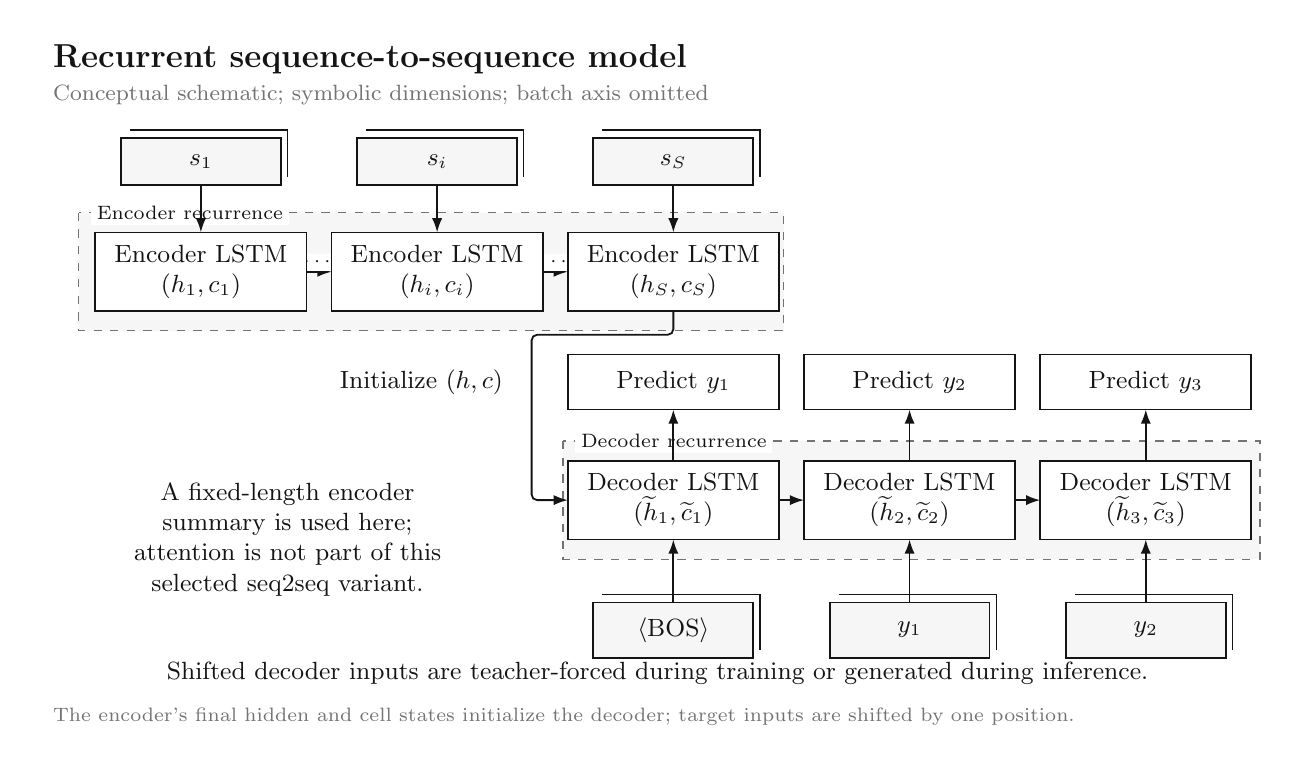
\begin{tikzpicture}[x=1cm,y=-1cm,font=\rmfamily,text=ink]

\path[use as bounding box] (0,0) rectangle (16,9);
\node[anchor=west,font=\large\bfseries] at (.2,.4) {Recurrent sequence-to-sequence model};
\node[anchor=west,font=\footnotesize,text=soft] at (.2,.85) {Conceptual schematic; symbolic dimensions; batch axis omitted};
\begin{pgfonlayer}{background}
\draw[groupbox] (0.65,2.35) rectangle (9.6,3.85);
\node[anchor=west,font=\scriptsize,fill=white,inner sep=2pt] at (0.8,2.35) {Encoder recurrence};
\draw[groupbox] (6.8,5.25) rectangle (15.649999999999999,6.75);
\node[anchor=west,font=\scriptsize,fill=white,inner sep=2pt] at (6.95,5.25) {Decoder recurrence};
\end{pgfonlayer}
\node[box,fill=wash,minimum width=2cm,minimum height=0.6cm,text width=1.75cm] (xa) at (2.2,1.7) {$s_{1}$};
\draw[ink,line width=.4pt] (1.3000000000000003,1.2999999999999998) -- (3.3000000000000003,1.2999999999999998) -- (3.3000000000000003,1.9);
\node[box,minimum width=2.65cm,minimum height=1.0cm,text width=2.4cm] (enca) at (2.2,3.1) {Encoder LSTM\\$(h_{1},c_{1})$};
\node[box,fill=wash,minimum width=2cm,minimum height=0.6cm,text width=1.75cm] (xb) at (5.2,1.7) {$s_{i}$};
\draw[ink,line width=.4pt] (4.3,1.2999999999999998) -- (6.3,1.2999999999999998) -- (6.3,1.9);
\node[box,minimum width=2.65cm,minimum height=1.0cm,text width=2.4cm] (encb) at (5.2,3.1) {Encoder LSTM\\$(h_{i},c_{i})$};
\node[box,fill=wash,minimum width=2cm,minimum height=0.6cm,text width=1.75cm] (xc) at (8.2,1.7) {$s_{S}$};
\draw[ink,line width=.4pt] (7.299999999999999,1.2999999999999998) -- (9.299999999999999,1.2999999999999998) -- (9.299999999999999,1.9);
\node[box,minimum width=2.65cm,minimum height=1.0cm,text width=2.4cm] (encc) at (8.2,3.1) {Encoder LSTM\\$(h_{S},c_{S})$};
\node[box,minimum width=2.65cm,minimum height=1.0cm,text width=2.4cm] (deca) at (8.2,6.0) {Decoder LSTM\\$(\widetilde h_{1},\widetilde c_{1})$};
\node[box,fill=wash,minimum width=2cm,minimum height=0.7cm,text width=1.75cm] (ina) at (8.2,7.65) {$\langle\mathrm{BOS}\rangle$};
\draw[ink,line width=.4pt] (7.299999999999999,7.200000000000001) -- (9.299999999999999,7.200000000000001) -- (9.299999999999999,7.9);
\node[box,minimum width=2.65cm,minimum height=0.7cm,text width=2.4cm] (outa) at (8.2,4.5) {Predict $y_{1}$};
\node[box,minimum width=2.65cm,minimum height=1.0cm,text width=2.4cm] (decb) at (11.2,6.0) {Decoder LSTM\\$(\widetilde h_{2},\widetilde c_{2})$};
\node[box,fill=wash,minimum width=2cm,minimum height=0.7cm,text width=1.75cm] (inb) at (11.2,7.65) {$y_1$};
\draw[ink,line width=.4pt] (10.299999999999999,7.200000000000001) -- (12.299999999999999,7.200000000000001) -- (12.299999999999999,7.9);
\node[box,minimum width=2.65cm,minimum height=0.7cm,text width=2.4cm] (outb) at (11.2,4.5) {Predict $y_{2}$};
\node[box,minimum width=2.65cm,minimum height=1.0cm,text width=2.4cm] (decc) at (14.2,6.0) {Decoder LSTM\\$(\widetilde h_{3},\widetilde c_{3})$};
\node[box,fill=wash,minimum width=2cm,minimum height=0.7cm,text width=1.75cm] (inc) at (14.2,7.65) {$y_2$};
\draw[ink,line width=.4pt] (13.299999999999999,7.200000000000001) -- (15.299999999999999,7.200000000000001) -- (15.299999999999999,7.9);
\node[box,minimum width=2.65cm,minimum height=0.7cm,text width=2.4cm] (outc) at (14.2,4.5) {Predict $y_{3}$};
\node[align=center,inner sep=0pt,outer sep=0pt,font=\small,minimum width=2.5cm,minimum height=0.5cm,text width=2.25cm] (note15) at (5.0,4.5) {Initialize $(h,c)$};
\node[align=center,inner sep=0pt,outer sep=0pt,font=\small,minimum width=5.6cm,minimum height=1.0cm,text width=5.35cm] (note16) at (3.3,6.5) {A fixed-length encoder summary is used here;\\attention is not part of this selected seq2seq variant.};
\node[align=center,inner sep=0pt,outer sep=0pt,font=\small,minimum width=14cm,minimum height=0.4cm,text width=13.75cm] (note17) at (8,8.2) {Shifted decoder inputs are teacher-forced during training or generated during inference.};
\begin{pgfonlayer}{background}
\draw[flow] (xa.south) -- (enca.north);
\draw[flow] (xb.south) -- (encb.north);
\draw[flow] (xc.south) -- (encc.north);
\draw[flow] (enca.east) -- (encb.west) node[midway,above,fill=white,inner sep=1.5pt,font=\scriptsize] {$\cdots$};
\draw[flow] (encb.east) -- (encc.west) node[midway,above,fill=white,inner sep=1.5pt,font=\scriptsize] {$\cdots$};
\draw[flow] (ina.north) -- (deca.south);
\draw[flow] (deca.north) -- (outa.south);
\draw[flow] (inb.north) -- (decb.south);
\draw[flow] (decb.north) -- (outb.south);
\draw[flow] (inc.north) -- (decc.south);
\draw[flow] (decc.north) -- (outc.south);
\draw[flow] (deca.east) -- (decb.west);
\draw[flow] (decb.east) -- (decc.west);
\draw[flow] (encc.south) -- (8.2,3.9) -- (6.4,3.9) -- (6.4,6.0) -- (deca.west);
\end{pgfonlayer}
\node[anchor=west,align=left,font=\scriptsize,text=soft,text width=15.6cm] at (.2,8.75) {The encoder's final hidden and cell states initialize the decoder; target inputs are shifted by one position.};
\end{tikzpicture}
\end{document}
